
%% bare_conf.tex
%% V1.3
%% 2007/01/11
%% by Michael Shell
%% See:
%% http://www.michaelshell.org/
%% for current contact information.
%%
%% This is a skeleton file demonstrating the use of IEEEtran.cls
%% (requires IEEEtran.cls version 1.7 or later) with an IEEE conference paper.
%%
%% Support sites:
%% http://www.michaelshell.org/tex/ieeetran/
%% http://www.ctan.org/tex-archive/macros/latex/contrib/IEEEtran/
%% and
%% http://www.ieee.org/

%%*************************************************************************
%% Legal Notice:
%% This code is offered as-is without any warranty either expressed or
%% implied; without even the implied warranty of MERCHANTABILITY or
%% FITNESS FOR A PARTICULAR PURPOSE! 
%% User assumes all risk.
%% In no event shall IEEE or any contributor to this code be liable for
%% any damages or losses, including, but not limited to, incidental,
%% consequential, or any other damages, resulting from the use or misuse
%% of any information contained here.
%%
%% All comments are the opinions of their respective authors and are not
%% necessarily endorsed by the IEEE.
%%
%% This work is distributed under the LaTeX Project Public License (LPPL)
%% ( http://www.latex-project.org/ ) version 1.3, and may be freely used,
%% distributed and modified. A copy of the LPPL, version 1.3, is included
%% in the base LaTeX documentation of all distributions of LaTeX released
%% 2003/12/01 or later.
%% Retain all contribution notices and credits.
%% ** Modified files should be clearly indicated as such, including  **
%% ** renaming them and changing author support contact information. **
%%
%% File list of work: IEEEtran.cls, IEEEtran_HOWTO.pdf, bare_adv.tex,
%%                    bare_conf.tex, bare_jrnl.tex, bare_jrnl_compsoc.tex
%%*************************************************************************

% *** Authors should verify (and, if needed, correct) their LaTeX system  ***
% *** with the testflow diagnostic prior to trusting their LaTeX platform ***
% *** with production work. IEEE's font choices can trigger bugs that do  ***
% *** not appear when using other class files.                            ***
% The testflow support page is at:
% http://www.michaelshell.org/tex/testflow/



% Note that the a4paper option is mainly intended so that authors in
% countries using A4 can easily print to A4 and see how their papers will
% look in print - the typesetting of the document will not typically be
% affected with changes in paper size (but the bottom and side margins will).
% Use the testflow package mentioned above to verify correct handling of
% both paper sizes by the user's LaTeX system.
%
% Also note that the "draftcls" or "draftclsnofoot", not "draft", option
% should be used if it is desired that the figures are to be displayed in
% draft mode.
%
\documentclass[conference]{IEEEtran}
% Add the compsoc option for Computer Society conferences.
%
% If IEEEtran.cls has not been installed into the LaTeX system files,
% manually specify the path to it like:
% \documentclass[conference]{../sty/IEEEtran}





% Some very useful LaTeX packages include:
% (uncomment the ones you want to load)


% *** MISC UTILITY PACKAGES ***
%
%\usepackage{ifpdf}
% Heiko Oberdiek's ifpdf.sty is very useful if you need conditional
% compilation based on whether the output is pdf or dvi.
% usage:
% \ifpdf
%   % pdf code
% \else
%   % dvi code
% \fi
% The latest version of ifpdf.sty can be obtained from:
% http://www.ctan.org/tex-archive/macros/latex/contrib/oberdiek/
% Also, note that IEEEtran.cls V1.7 and later provides a builtin
% \ifCLASSINFOpdf conditional that works the same way.
% When switching from latex to pdflatex and vice-versa, the compiler may
% have to be run twice to clear warning/error messages.






% *** CITATION PACKAGES ***
%
%\usepackage{cite}
% cite.sty was written by Donald Arseneau
% V1.6 and later of IEEEtran pre-defines the format of the cite.sty package
% \cite{} output to follow that of IEEE. Loading the cite package will
% result in citation numbers being automatically sorted and properly
% "compressed/ranged". e.g., [1], [9], [2], [7], [5], [6] without using
% cite.sty will become [1], [2], [5]--[7], [9] using cite.sty. cite.sty's
% \cite will automatically add leading space, if needed. Use cite.sty's
% noadjust option (cite.sty V3.8 and later) if you want to turn this off.
% cite.sty is already installed on most LaTeX systems. Be sure and use
% version 4.0 (2003-05-27) and later if using hyperref.sty. cite.sty does
% not currently provide for hyperlinked citations.
% The latest version can be obtained at:
% http://www.ctan.org/tex-archive/macros/latex/contrib/cite/
% The documentation is contained in the cite.sty file itself.






% *** GRAPHICS RELATED PACKAGES ***
%
\ifCLASSINFOpdf
  % \usepackage[pdftex]{graphicx}
  % declare the path(s) where your graphic files are
  % \graphicspath{{../pdf/}{../jpeg/}}
  % and their extensions so you won't have to specify these with
  % every instance of \includegraphics
  % \DeclareGraphicsExtensions{.pdf,.jpeg,.png}
\else
  % or other class option (dvipsone, dvipdf, if not using dvips). graphicx
  % will default to the driver specified in the system graphics.cfg if no
  % driver is specified.
  % \usepackage[dvips]{graphicx}
  % declare the path(s) where your graphic files are
  % \graphicspath{{../eps/}}
  % and their extensions so you won't have to specify these with
  % every instance of \includegraphics
  % \DeclareGraphicsExtensions{.eps}
\fi
% graphicx was written by David Carlisle and Sebastian Rahtz. It is
% required if you want graphics, photos, etc. graphicx.sty is already
% installed on most LaTeX systems. The latest version and documentation can
% be obtained at: 
% http://www.ctan.org/tex-archive/macros/latex/required/graphics/
% Another good source of documentation is "Using Imported Graphics in
% LaTeX2e" by Keith Reckdahl which can be found as epslatex.ps or
% epslatex.pdf at: http://www.ctan.org/tex-archive/info/
%
% latex, and pdflatex in dvi mode, support graphics in encapsulated
% postscript (.eps) format. pdflatex in pdf mode supports graphics
% in .pdf, .jpeg, .png and .mps (metapost) formats. Users should ensure
% that all non-photo figures use a vector format (.eps, .pdf, .mps) and
% not a bitmapped formats (.jpeg, .png). IEEE frowns on bitmapped formats
% which can result in "jaggedy"/blurry rendering of lines and letters as
% well as large increases in file sizes.
%
% You can find documentation about the pdfTeX application at:
% http://www.tug.org/applications/pdftex





% *** MATH PACKAGES ***
%
%\usepackage[cmex10]{amsmath}
% A popular package from the American Mathematical Society that provides
% many useful and powerful commands for dealing with mathematics. If using
% it, be sure to load this package with the cmex10 option to ensure that
% only type 1 fonts will utilized at all point sizes. Without this option,
% it is possible that some math symbols, particularly those within
% footnotes, will be rendered in bitmap form which will result in a
% document that can not be IEEE Xplore compliant!
%
% Also, note that the amsmath package sets \interdisplaylinepenalty to 10000
% thus preventing page breaks from occurring within multiline equations. Use:
%\interdisplaylinepenalty=2500
% after loading amsmath to restore such page breaks as IEEEtran.cls normally
% does. amsmath.sty is already installed on most LaTeX systems. The latest
% version and documentation can be obtained at:
% http://www.ctan.org/tex-archive/macros/latex/required/amslatex/math/





% *** SPECIALIZED LIST PACKAGES ***
%
%\usepackage{algorithmic}
% algorithmic.sty was written by Peter Williams and Rogerio Brito.
% This package provides an algorithmic environment fo describing algorithms.
% You can use the algorithmic environment in-text or within a figure
% environment to provide for a floating algorithm. Do NOT use the algorithm
% floating environment provided by algorithm.sty (by the same authors) or
% algorithm2e.sty (by Christophe Fiorio) as IEEE does not use dedicated
% algorithm float types and packages that provide these will not provide
% correct IEEE style captions. The latest version and documentation of
% algorithmic.sty can be obtained at:
% http://www.ctan.org/tex-archive/macros/latex/contrib/algorithms/
% There is also a support site at:
% http://algorithms.berlios.de/index.html
% Also of interest may be the (relatively newer and more customizable)
% algorithmicx.sty package by Szasz Janos:
% http://www.ctan.org/tex-archive/macros/latex/contrib/algorithmicx/




% *** ALIGNMENT PACKAGES ***
%
%\usepackage{array}
% Frank Mittelbach's and David Carlisle's array.sty patches and improves
% the standard LaTeX2e array and tabular environments to provide better
% appearance and additional user controls. As the default LaTeX2e table
% generation code is lacking to the point of almost being broken with
% respect to the quality of the end results, all users are strongly
% advised to use an enhanced (at the very least that provided by array.sty)
% set of table tools. array.sty is already installed on most systems. The
% latest version and documentation can be obtained at:
% http://www.ctan.org/tex-archive/macros/latex/required/tools/


%\usepackage{mdwmath}
%\usepackage{mdwtab}
% Also highly recommended is Mark Wooding's extremely powerful MDW tools,
% especially mdwmath.sty and mdwtab.sty which are used to format equations
% and tables, respectively. The MDWtools set is already installed on most
% LaTeX systems. The lastest version and documentation is available at:
% http://www.ctan.org/tex-archive/macros/latex/contrib/mdwtools/


% IEEEtran contains the IEEEeqnarray family of commands that can be used to
% generate multiline equations as well as matrices, tables, etc., of high
% quality.


%\usepackage{eqparbox}
% Also of notable interest is Scott Pakin's eqparbox package for creating
% (automatically sized) equal width boxes - aka "natural width parboxes".
% Available at:
% http://www.ctan.org/tex-archive/macros/latex/contrib/eqparbox/





% *** SUBFIGURE PACKAGES ***
%\usepackage[tight,footnotesize]{subfigure}
% subfigure.sty was written by Steven Douglas Cochran. This package makes it
% easy to put subfigures in your figures. e.g., "Figure 1a and 1b". For IEEE
% work, it is a good idea to load it with the tight package option to reduce
% the amount of white space around the subfigures. subfigure.sty is already
% installed on most LaTeX systems. The latest version and documentation can
% be obtained at:
% http://www.ctan.org/tex-archive/obsolete/macros/latex/contrib/subfigure/
% subfigure.sty has been superceeded by subfig.sty.



%\usepackage[caption=false]{caption}
%\usepackage[font=footnotesize]{subfig}
% subfig.sty, also written by Steven Douglas Cochran, is the modern
% replacement for subfigure.sty. However, subfig.sty requires and
% automatically loads Axel Sommerfeldt's caption.sty which will override
% IEEEtran.cls handling of captions and this will result in nonIEEE style
% figure/table captions. To prevent this problem, be sure and preload
% caption.sty with its "caption=false" package option. This is will preserve
% IEEEtran.cls handing of captions. Version 1.3 (2005/06/28) and later 
% (recommended due to many improvements over 1.2) of subfig.sty supports
% the caption=false option directly:
%\usepackage[caption=false,font=footnotesize]{subfig}
%
% The latest version and documentation can be obtained at:
% http://www.ctan.org/tex-archive/macros/latex/contrib/subfig/
% The latest version and documentation of caption.sty can be obtained at:
% http://www.ctan.org/tex-archive/macros/latex/contrib/caption/




% *** FLOAT PACKAGES ***
%
%\usepackage{fixltx2e}
% fixltx2e, the successor to the earlier fix2col.sty, was written by
% Frank Mittelbach and David Carlisle. This package corrects a few problems
% in the LaTeX2e kernel, the most notable of which is that in current
% LaTeX2e releases, the ordering of single and double column floats is not
% guaranteed to be preserved. Thus, an unpatched LaTeX2e can allow a
% single column figure to be placed prior to an earlier double column
% figure. The latest version and documentation can be found at:
% http://www.ctan.org/tex-archive/macros/latex/base/



%\usepackage{stfloats}
% stfloats.sty was written by Sigitas Tolusis. This package gives LaTeX2e
% the ability to do double column floats at the bottom of the page as well
% as the top. (e.g., "\begin{figure*}[!b]" is not normally possible in
% LaTeX2e). It also provides a command:
%\fnbelowfloat
% to enable the placement of footnotes below bottom floats (the standard
% LaTeX2e kernel puts them above bottom floats). This is an invasive package
% which rewrites many portions of the LaTeX2e float routines. It may not work
% with other packages that modify the LaTeX2e float routines. The latest
% version and documentation can be obtained at:
% http://www.ctan.org/tex-archive/macros/latex/contrib/sttools/
% Documentation is contained in the stfloats.sty comments as well as in the
% presfull.pdf file. Do not use the stfloats baselinefloat ability as IEEE
% does not allow \baselineskip to stretch. Authors submitting work to the
% IEEE should note that IEEE rarely uses double column equations and
% that authors should try to avoid such use. Do not be tempted to use the
% cuted.sty or midfloat.sty packages (also by Sigitas Tolusis) as IEEE does
% not format its papers in such ways.





% *** PDF, URL AND HYPERLINK PACKAGES ***
%
%\usepackage{url}
% url.sty was written by Donald Arseneau. It provides better support for
% handling and breaking URLs. url.sty is already installed on most LaTeX
% systems. The latest version can be obtained at:
% http://www.ctan.org/tex-archive/macros/latex/contrib/misc/
% Read the url.sty source comments for usage information. Basically,
% \url{my_url_here}.

\usepackage{graphicx} %----------------------- For using images
\DeclareGraphicsExtensions{.pdf,.png,.jpg} %-------- Extensions for images
\usepackage{color}



% *** Do not adjust lengths that control margins, column widths, etc. ***
% *** Do not use packages that alter fonts (such as pslatex).         ***
% There should be no need to do such things with IEEEtran.cls V1.6 and later.
% (Unless specifically asked to do so by the journal or conference you plan
% to submit to, of course. )


% correct bad hyphenation here
\hyphenation{op-tical net-works semi-conduc-tor}


\begin{document}
%
% paper title
% can use linebreaks \\ within to get better formatting as desired
\title{A novel Classification-based Hybrid IDS}


% author names and affiliations
% use a multiple column layout for up to three different
% affiliations
\author{\IEEEauthorblockN{Oscar Rodas H., Jose A Alvarez Aldana and Gerardo Morales}
\IEEEauthorblockA{RLICT / Universidad Galileo\\
7Av. Final Calle Dr. Eduardo Suger Zona 10\\
Guatemala, Guatemala\\
Email: {\{orodas,josealfredo1515,gmorales\}@galileo.edu}}
\and
\IEEEauthorblockN{Stephane Maag}
\IEEEauthorblockA{Institut Mines-Telecom / Telecom SudParis\\
CNRS UMR 5157\\
9, rue Charles Fourier, 91011, EVRY Cedex, France\\
Email: {Stephane.Maag@telecom-sudparis.eu}}
}

% make the title area
\maketitle


\begin{abstract}
%\boldmath
For years, the IDS industry has worked on bringing a solution to anomaly-based attacks on computer networks. The main concerns related to the IDS implementations have been: low detection rate of anomaly-based attacks that causes low usability and high rate of false positives that causes low acceptability. Researchers in the field of IT have proposed different approaches using numerous techniques to improve these rates.  This paper presents an approach based on the problematic faced by networks when anomaly-based attacks emerge.  The approach proposes a novel framework based on analyzing real-time information and classifying traffic in a binary way, \emph{legitimate}  or an \emph{intrusion}. Log information will be correlated with the same customized format, filtered and stored in mongoDB by Collaborative Intrusion  Detection System (CIDS). This CIDS will be the main entity for examining correlation in the log information.  While correlating the information with the help of mongoDB, the framework will be able to rapidly determine the existence of anomaly-based intrusions and will notify the different entities in the network about the intrusion. The framework will dynamically adapt to the kind of traffic present in the network. The case study for this paper will be based on the typically Brute Force Attack launched to any server running the SSH protocol. The SSH protocol was chosen because it is the default remote protocol sysadmins use for remote connections on networks worldwide.
\end{abstract}

% IEEEtran.cls defaults to using nonbold math in the Abstract.
% This preserves the distinction between vectors and scalars. However,
% if the conference you are submitting to favors bold math in the abstract,
% then you can use LaTeX's standard command \boldmath at the very start
% of the abstract to achieve this. Many IEEE journals/conferences frown on
% math in the abstract anyway.

% no keywords




% For peer review papers, you can put extra information on the cover
% page as needed:
% \ifCLASSOPTIONpeerreview
% \begin{center} \bfseries EDICS Category: 3-BBND \end{center}
% \fi
%
% For peerreview papers, this IEEEtran command inserts a page break and
% creates the second title. It will be ignored for other modes.
\IEEEpeerreviewmaketitle

\section{Introduction}
Private and public networks, like The Internet, have become a place where people do business, check email, perform transactions and bring everyday life activities to a virtual environment, making it important to follow the three pillars of Information Security, which are, \emph{confidentiality, integrity and availability}.  When a transaction fails to meet this kind of compliance, it means that the network is vulnerable to a security breach. To mitigate these kinds of problems, companies need a comprehensive security system on their network. Protection should start with a component that runs analysis on traffic, coming in and out of it, and that also has the capacity to classify this traffic as legitimate or intrusion. Classifying traffic should be handled by an Intrusion Detection System (IDS) on the network. The IDS industry has developed different approaches for the intrusion detection in networks.  %Classification of IDSs can be made by the techniques they use to detect anomalies, by the kind of implementation, by the way they manage and classify information, among others. 

Commonly, researchers working in Information Security \cite{deshmukhDetectionOfAttacks} \cite{chen2010efficientnetworkintrusion} classify IDSs into two different types depending on the kind of implementation:
\begin{itemize}
\item \textbf{HIDS (Host-based Intrusion Detection System)}:  This IDS is installed on every device (host) that is connected to a network.  Its purpose is to capture and analyze network data from the device.  
\item \textbf{NIDS (Network-based Intrusion Detection System)}: This IDS is either installed at the network gateway, with the purpose of analyzing traffic on all devices in the network.  The IDS will then inspect packets and will be able to determine an attack before it reaches the endpoints.
\end{itemize}

Various factors should be considered when deciding the best place in the network to implement an IDS solution.  \emph{Chen et al.} \cite{chen2010efficientnetworkintrusion} state that HIDSs imply high costs of installation and maintenance.  NIDSs imply a single point of failure existing in the architecture designed for implementing security on the network.  NIDSs also imply a single resource on the network that spends a lot of time processing and analyzing packet content and could degrade the system performance. Deciding the right spot to implement the IDS will determine if it should be installed either at a centralized point or at a particular host.  NIDS,  installed on a gateway, router or server are able to analyze all the traffic incoming or outgoing to the network.  HIDS installed on particular host (computer, laptop, etc.) are able to analyze its particular traffic.  In both implementations the IDS will always be analyzing traffic and sending alarms if any intrusion attack has been detected.

IDS can also be categorized based on the approach they use to determine if traffic can be considered as ``legitimate" or ``anomalous" \cite{deshmukhDetectionOfAttacks} \cite{garcia2009anomaly}. These different approaches are based on two main techniques. \emph{a.) Misuse Detection}:  This detection is based on the use of signature-based intrusion detection.  The packet is first examined to determine if it can be categorized as an anomaly. If the packet does not comply with any of the signatures, then it can be categorized as ``legitimate" traffic.  \emph{b.) Anomaly Detection}: This detection is based on the use of a profile of a user, server or network that after some criteria is denoted as ``legitimate". Starting from this profile, every other traffic that does not comply with the profile will be considered an anomaly.

Even though, the IDSs in the recent years were improved by the intrusion detection industries, they still have two major concerns \cite{thomas2013application}: \textit{Low detection rate of anomaly-based intrusion attacks} that causes low usability and \textit{High rate of false positives} that causes low acceptability.\\

There has been numerous approaches using different techniques to try to improve these rates.  Recently, researchers have proposed approaches using machine learning techniques to detect intrusions \cite{tsai2009intrusion} \cite{aydin2009hybrid} \cite{panda2012hybrid} \cite{thomas2013application} \cite{bajaj2013improving}. Their main contribution is the implementation of hybrid approaches that detect anomaly-based intrusions after filtering traffic that complied with signature-based techniques. Other researches have approaches that correlate information from different traffic observations to determine anomaly-based attacks after long periods of time \cite{tsai2010triangle}.              

Regarding new kinds of attacks like coordinated attacks, \textit{{Collaborative Intrusion Detection (CIDS)}} Systems have been a solution to address this kind of problem. A survey by \textit{Zhou et al.} \cite{zhou2010survey} describes the need of having various IDSs in a network collaborating to correlate log information from different parts of a network. Analyzing correlated data from different logs will make easier the detection of coordinated attacks like large-scale stealthy scans, worm outbreaks and Distributed Denial-of-Service (DDos) attacks. Contrary to having isolated IDSs that only monitor a limited portion of the network and make extremely difficult the detection of these kind of attacks.  

The main contributions of this paper after examining different approaches to detect anomaly-based attacks are:
\begin{itemize}
\item \textit{Definition of a novel framework to detect anomaly-based intrusion attacks}.  The framework is based on anomaly-based intrusion detection systems (A-IDS) embedded in different areas of a distributed system. All A-IDS send log information to a central repository with mongoDB \cite{mongoDB}, a database, for further collaborative anomaly-based intrusion attack detection. This correlation is handled by a Collaborative Intrusion Detection System (CIDS) analyzing all data in real time. 
\item \textit{A more precise traffic classification methodology}. While correlating all the information of the different IDSs installed on the network, the framework enables to classify traffic in a binary way, as \textit{legitimate} or as an  \textit{intrusion}.
\end{itemize}

The remainder of the paper is organized as follows.  In Section \ref{rw}, we review the related work of other researchers and how they motivated and help the research presented in this paper.  In Section \ref{framework}, we describe our novel framework and in Section \ref{exp} we present the experimental studies and the results obtained with our testbed. We conclude and give perspectives in Section \ref{conclusion}.

\section{Related Work}
\label{rw}

%The work done in the subject has been focused on techniques that would increasing the anomaly-based detection rate and to decrease the false positive rate.  Other works have concentrated on proposing new approaches for the implementation of IDSs. In the following, we cite relevant papers from which we got inspired.

%The next subsections will describe most of the previous research done that inspired this work.

\subsection{Machine Learning Techniques}
In \cite{garcia2009anomaly},  \textit{Garcia-Teodoro et al.} described the techniques, systems and challenges in anomaly-based network intrusion detection.  They mention the existence of the IDWG (Intrusion Detection Working Group) that was based on the CIDF (Common Intrusion Detection Framework)\footnote{http://www.ietf.org/wg-descriptions/cidf.desc.txt}.  

\textit{Tsai et al.} \cite{tsai2009intrusion} %describe the use of machine learning techniques for intrusion detection.  The amount of machine learning algorithms used for intrusion detection will determine if the approach uses single, hybrid or ensemble classifiers.  The review
examined 55 related studies based on the type of classifier. 
%It concluded that the research at that point still had to advanced. 
The review promoted the research of combining hybrid and ensemble classifiers to create better IDS that would increase the detection rates on anomalous traffic going through networks.  Furthermore, it also mentioned the importance of feature selection for analyzing traffic and reducing the workload for analysis by IDSs.

\subsection{Hybrid Techniques} 

The proposal of \textit{Aydin et al.} \cite{aydin2009hybrid} describes a hybrid approach, concatenating anomaly-based and misuse intrusion detections systems.  This approach delivered results that increased the anomaly detection rate in SNORT \cite{SNORT}. %from 27 attacks detected by itself to a 146 detected after the concatenation of all the systems.  
Our approach differs from the way of implementing the hybrid IDS.  This implementation is based on a single Network IDS, which makes the a solution to be based on a single point of failure. Additionally, the implementation was only tested on an \textit{IDEVAL} \cite{IDEVAL} testbed and not on real-time traffic, unlike our approach.

\subsection{Other Techniques}

One of the challenging issues of network and system management operators is the every day dealing with huge amount of alerts generated~\cite{modelbasedsurveySalahMD13}.  These alerts can obfuscate the appearance of anomalous behaviors. The use of alert correlation has become one of the most popular resources used for detecting collaborative attacks. Our framework deals with the problem of scalability, it can handle as much network entities as the distributed system needs to be consider secure.        
 
\textit{Chen et al.} \cite{chen2010efficientnetworkintrusion} describe an efficient network intrusion detection approach based on a Lightweight Network Intrusion Detection system (LNID). Our approach differs from their solution that is based on a single Network IDS.

\textit{Zhou et al.} \cite{zhou2010survey} mentions that the major problem is \emph{Coordinated Attacks}, which are a large-scale stealthy scans, worm outbreaks and distributed denial-of-service (DDoS) attacks that occurred in different networks at the same time. In their survey they focus on two important factors for detecting anomaly-based intrusions:
\begin{itemize}
\item \textit{Collaborative Intrusion Detection Systems (CIDSs)} and their architecture.
\item \textit{Alert Correlation Algorithms} to detect this kind of attacks.
\end{itemize}

It is mentioned that every attack has a common stage in which all traffic either comes from the same source (stealthy scans or worm outbreaks) or the traffic goes to a particular host or server (DDoS attacks). Researchers describe that improving the techniques for HIDSs or NIDSs can help detect anomaly-based traffic in a more precise manner. Also, that there is a need to correlate all the logs of the different IDSs on large-scale networks, like the Internet, to determine new kind of attacks. Our approach enhances this feature by having a CIDS that will only be managing the correlation of the logs and, in this first approach, our correlation is based on the source IP address of the attacks. 

Table 1 highlights that neither a Centralized nor Hierarchical approach for system architecture is the best for collaborative intrusion detection.  Our approach takes into consideration the advantages of the Centralized and Hierarchical approach mentioned before and implements a hybrid architecture. This hybrid architecture is based on hierarchy and centralization.  Hierarchy will have two different phases to detect anomalous traffic and will be implemented as follows:
\begin{itemize}
\item \textbf{Phase 1:} IDSs will be installed across the network and will be responsible for intrusion detections at their particular areas (host or network).  
\item \textbf{Phase 2:} All log information will be sent to a CIDS that will manage the correlation of the information to determine the possibility of coordinated attacks present in the network and to classify traffic as \emph{legitimate} or as an \emph{intrusion}.
\end{itemize}

\textit{Centralization} is used for managing the correlation of log information to determine the possibility of collaborative intrusion attacks.  The merging of both architectures into this novel hybrid approach makes the whole new framework to be able to protect the network without having a single point of failure, like a centralized approach.  Moreover, we drastically save processing power and would not have the same detection speed and capacity, like a hierarchical approach.  Detailed information can be found in Table \ref{sumcids}.
%------------table 
\begin{table}[h!]
\caption{Summary of CIDS Research - System Architecture Point of View}
\label{sumcids}
\begin{tabular}{p{2.5cm}p{2.3cm}p{2.8cm}}
%\toprule
%\multicolumn{3}{l}{System Architecture} \\
\hline
Classification & Advantages & Disadvantages \\
\hline
Centralized & Efficient for small scale cooperation & Single point of failure; Poor scalability \\
Hierarchical & No single point of failure & Limited Scalability; Reduced detection capacity during attacks \\
Distributed & No single point of failure; Better scalability & Load imbalance during attacks; Uncertain detection accuracy; Simplistic alert correlation \\
\hline
\end{tabular}
\end{table}

In this work, we are interested in describing a new approach to handle collaborative anomaly-based intrusion attacks. The proposed framework has different IDSs being installed all over the distributed system protected.  These IDSs will send log information to the Collaborative Intrusion Detection System (CIDS), which is the central repository responsible for the correlation of all the traffic incoming and outgoing from the whole network. By implementing the IDSs in this architecture the framework can:
\begin{itemize}
\item Analyze data in real-time about the whole network and search for anomaly-based intrusion attacks. The results are obtained in a fast way using mongoDB \cite{mongoDB} for compilation.
\item Correlate all the logs from the network to determine the existence of collaborative anomaly-based intrusion attack. If an attack is detected in the network, the framework will automatically block the source IP address and inform the rest of the network entities to block that IP address. This kind of information sent to other network entities and the automatic process of determining an attack in the network by the framework, is what gives this novel framework a sense of intelligence. 
\item Assure a high detection rate based on the log information of the distributed IDSs and low false alarm rate (correlation of log information and classification of legitimate and anomalous traffic).
\end{itemize} 
%As a future work, the framework will be complemented having the capacity to reconfigure its normal profile using machine learning techniques and with this information be able to define new collaborative intrusion attacks. Important to highlight that the new classification of traffic will be shared with the rest of the IDS to make a more precise binary classification in further analyses.

\section{Hybrid Intrusion Detection System}
\label{framework}
\subsection{IB Framework}
Figure \ref{fw} describes the proposed framework for \emph{correlative anomaly-based intrusion detection} in a network.  The dash lines indicate the connections inside the network for operation.  The solid bold lines indicate the connections inside the network for collaborative intrusion detection.
\begin{figure}[h!]
\caption{Proposed Framework}
\label{fw}
\centering
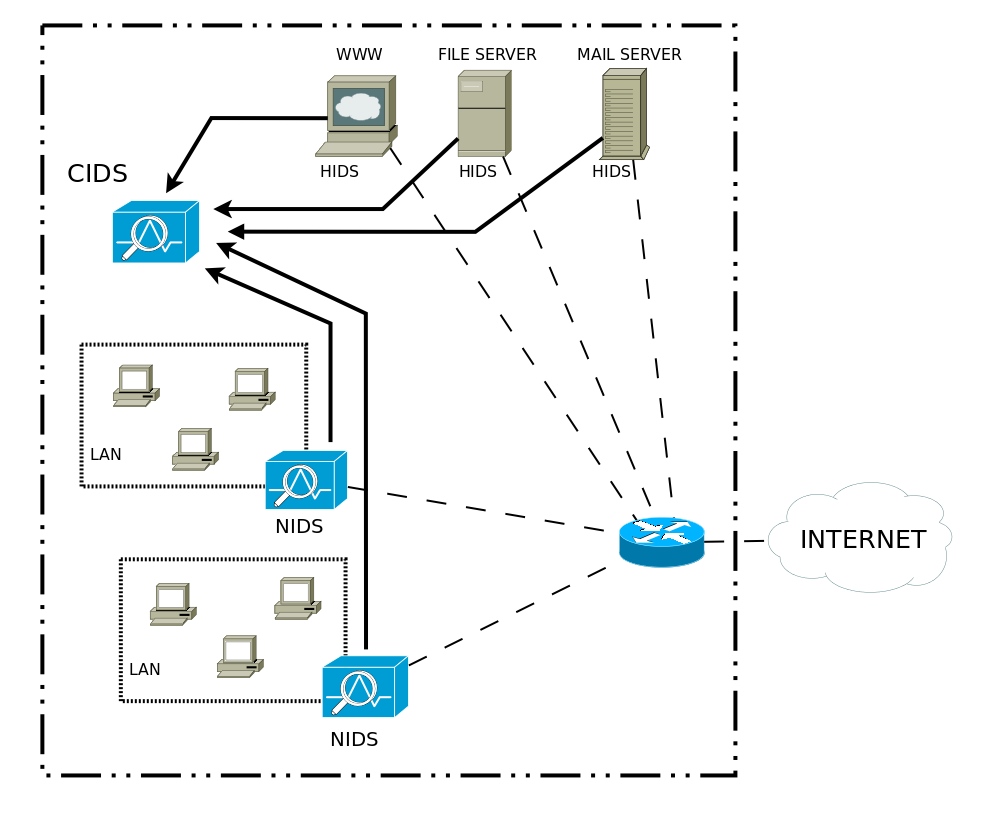
\includegraphics[scale=0.12]{framework-v3}
\end{figure}

The framework is composed by the following components:
\begin{itemize}
\item \textbf{NIDS:} The NIDS in the network is responsible for stopping intrusion attacks in the LAN area of the network they were installed for protecting. Installing NIDS to secure a network is easier and the cost of installation and maintenance are decreased. These NIDS send log information to the \emph{Collaborative Intrusion Detection System (CIDS)} installed on the network.
\item \textbf{HIDS:} The HIDS in the network is responsible for stopping intrusion attacks for each server or host in the network. By having each server or host with its own HIDS will assure that each of the services used in the network will be protected. Another benefit will be to prevent a bottleneck for the services attended by the servers.
\item \textbf{CIDS:} The CIDS is the IDS specialized to correlate log information between the above mentioned components.
\item \textbf{IB Framework:} The IB framework is our novel approach to be able to detect anomaly-based intrusion packets. This framework correlates all the information sent by the different NIDSs or HIDSs mentioned above. The correlation will be managed and centralized in the CIDS. The framework is able to analyze packets in real time and will have the capacity to classify them as either \emph{legitimate } or an \emph{intrusion}. The IB framework will classify all the packets based on a \emph{trust coefficient (TC)}. This TC at first marks every single incoming packet in an "unknown" state. After more incoming traffic of the same kind will be present on the network, and its behavior has been analyzed, the TC will converge to a \emph{legitimate} or \emph{intrusion} state.
\end{itemize}

As a summary, the input to the IDSs will be the incoming traffic passing through each one.  Each IDS will be responsible for protecting the part of the network it guards. The log information capture by each of the IDSs will then be sent to the CIDS to correlate it.  The CIDS will manage the information in a database for easier access and doing queries. To be able to acquire better results on analyzing the data, the solution is implemented using mongoDB. The CIDS processes lots of information because all the log information from each NIDS or HIDS have to be correlated and then determine the possibility of a coordinated / collaborative attack.  The information managed by all the IDS will be in the same format to facilitate its processing. %As an example of the changes made to the log information and how this eases analyzing, parsing and correlating of the information, we give a part of the logs provided by some of the servers and already centralized in the CIDS.

%{\footnotesize{
%\begin{verbatim}

%Sep  7 13:58:48 monserver ip-dst:192.168.8.10 6 
%info sshd[25422]: Failed password for 
%invalid user root from 115.238.227.66 port 1962 ssh2
%Sep  7 13:58:48 monserver ip-dst:192.168.8.10 6 
%info sshd[25420]: Failed password for invalid user 
%united from 84.242.76.66 port 53799 ssh2
%Sep  7 13:58:48 monserver ip-dst:192.168.8.10 6 
%info sshd[25420]: Received disconnect from 
%84.242.76.66: 11: Bye Bye [preauth]
%Sep  7 13:58:48 monserver ip-dst:192.168.8.10 6 
%info sshd[25424]: Connection from 84.242.76.66 
%port 55439
%Sep  7 13:58:48 elec-web ip-dst:192.168.8.20 6 
%info sshd[4226]: Invalid user sciops 
f%rom 84.242.76.66
%Sep  7 13:58:48 elec-web ip-dst:192.168.8.20 6 
%info sshd[4224]: Failed password for invalid user 
%root from 115.238.227.66 port 1973 ssh2
%\end{verbatim}
%}}

\subsection{The Implemented Framework}

\subsubsection{Description}
The implementation of IB framework is simplified for this paper. The scenario was built to show the methodology proposed to rapidly decide if an ssh login attempt can be consider \emph{legitimate} or an  \emph{intrusion}. The scenario shows two important topics to be considered. a.) The importance of log correlation and how this helps to determine anomaly-distributed attacks and b.) How the proposed framework determines that a login attempt is either  \emph{legitimate} or an \emph{intrusion}. The classification method use in the IB framework is based to ensure that the anomaly detection rate is increased and the false positive rate is decreased.

In the scenario, there are three servers: a.) A web server (192.168.8.20) with 10 virtual hosts, b.) A server (192.168.8.10) that has web and file services running, c.) A server (192.168.8.66) that has a web service running and is used as the correlation server. This server is the most powerful in resources. For this scenario it uses 4 vCPUs and 8GB of RAM. and a d.) Host (192.168.8.143) running an IDS and some basic services.

\begin{figure}[h!]
\caption{\textbf{Implemented Scenario}}
\label{impscen}
\centering
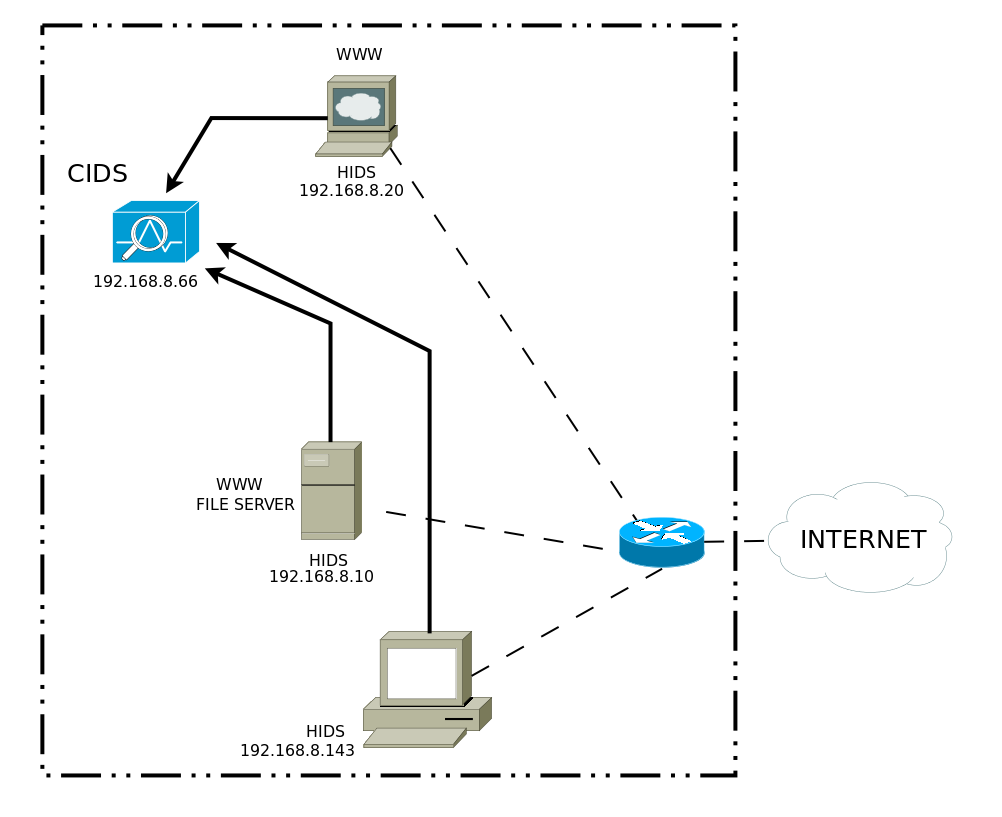
\includegraphics[scale=0.12]{framework-v5} 
\end{figure}

Our framework has been implemented with regards to anomaly intrusion detection for brute force attacks on a network with SSH capabilities on its hosts. Based on the logs of the network entities such as servers, appliances or end user clients, the data will be stored and analyzed. For this first approach, the key parameters are the source IP address to whom the login attempt was directed and the trust coefficient (TC) calculated after each new login attempt. The centralized and correlated logs will be the information needed to extract and filter login attempts by its source IP address. The trust coefficient (TC) is the value that determines if the login attempt is considered (i) an unknown package (first time information is in the framework), (ii) regular access (legitimate) or (iii) an intrusion. 
The trust level of a source IP address doing a login attempt is determine, manage and filter depending on the trust coefficient (TC) that was describe above and how it responds to two thresholds, a \emph{minimum (MINTHR)} and a \emph{maximum (MAXTHR)} present in the decision making. The characteristics of these thresholds are:
\begin{itemize}
\item MINTHR and MAXTHR are in the range [0, 100],
\item MAXTHR\textgreater MINTHR.
\end{itemize}
These thresholds will be of use to determine the status of a login attempt in one of the next classifications:
\begin{itemize}
\item If the trust coefficient is between 100 and MAXTHR it means that the login attempt is consider a \emph{legitimate authentication}. In this case, the source IP address doing the login attempt is considered to have \emph{high trust level}.
\item If the trust coefficient is between MAXTHR and MINTHR it means that the login attempt is an unknown authentication state. This might happen when the source IP address is added for the first time to the framework analysis or still gaining / losing its trust level.
\item If the trust coefficient is between MINTHR and 0 the login attempt is considered part of an attack and the source IP address has a low trust level. Automatically the framework will add the source IP address to a list of IPs that should be blocked. A notification will be sent to every other network entity to inform them about this new source IP address that is consider to be part of an attack and that has to be blocked. By implementing this notification information to all the network entities in the network and reconfiguring their IDSs, the whole framework projects a sense of intelligence by being able to reconfigure its behavior to new anomaly intrusion behaviors that will be considered attacks.
\end{itemize}

\begin{figure}[h!]
\caption{\textbf{Framework Flowchart}}
\label{frmflowchart}
\centering
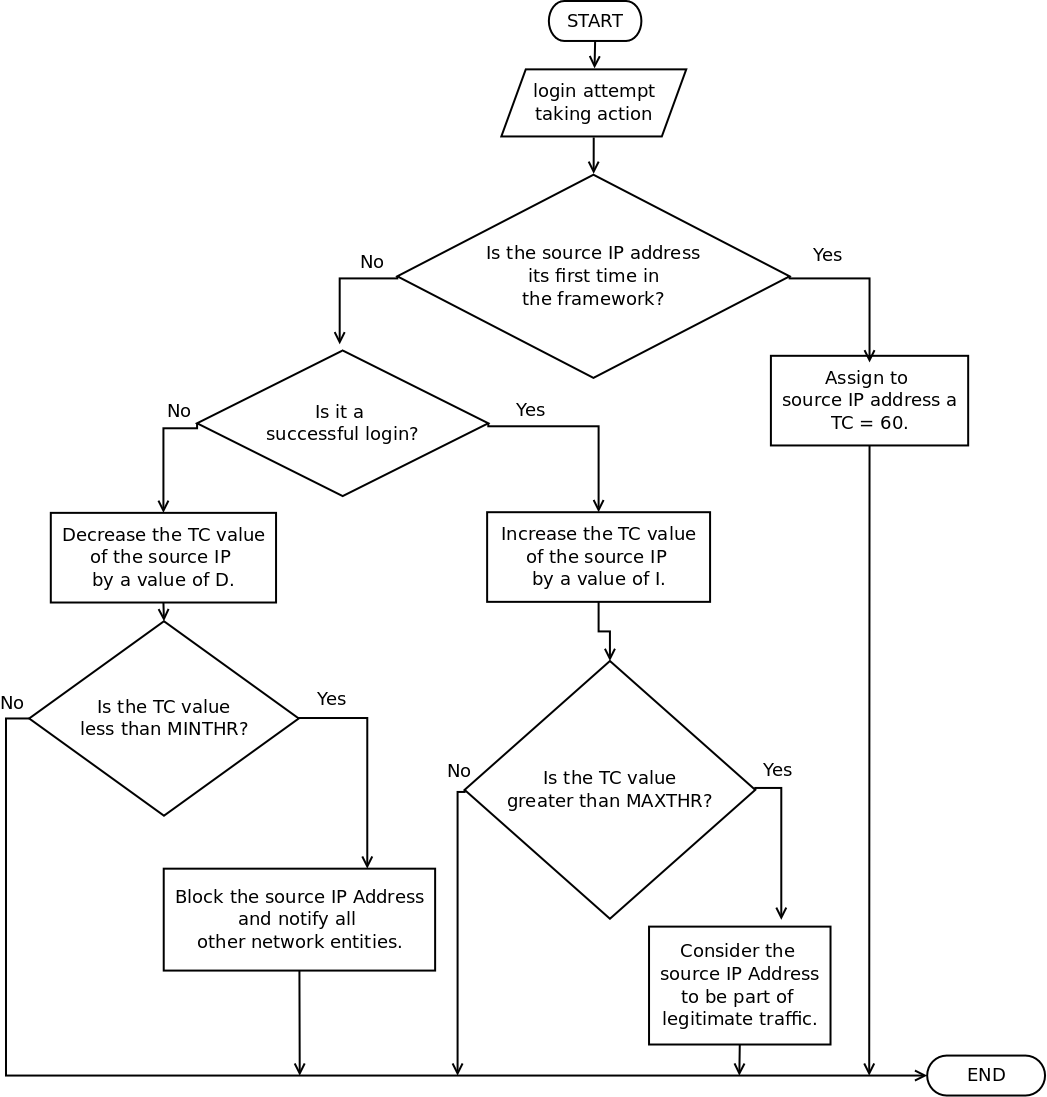
\includegraphics[scale=0.12]{framework-flowchart} 
\end{figure}
The trust coefficient will either increase or decrease during the login attempts. The increasing or decreasing values are considered I and D, respectively. The computation done for determining an increment or decrement of the trust coefficient is based on the fact that an ssh login attempt can be either considered as a \emph{successful login} or a \emph{failed login}. \emph{P} is a coefficient that will be useful to determine the relationship between a successful login or a failed login. Define \emph{D = P*I}, the greater this P value is, the more secure the sysadmin or IT manager wants its hosts to be. P value should always be greater than 0.

\subsubsection{An Example}
At first, a source IP address doing a login attempt will be considered \emph{unknown}. The second and next login attempts will be considered either a successful login or a failed login.  If the login attempt is a \emph{successful login}, the trust coefficient (TC) will increase by a value of I. If the login attempt is consider a \emph{failed login}, the trust coefficient (TC) will decrease by a value of D. Notice that since D will always be greater than I, it will be easier for the trust coefficient (TC) to fall into the zone considered as an intrusion rather than into a legitimate zone. \\
After determining the temporal TC value of each login attempt as mentioned before, the framework will determine the status of the source IP address regarding its last login attempt. Any source IP address analyze by the framework could either be in one of the next statuses. a.) Still at an \emph{unknown stage} if the TC value is between the MAXTHR and the MINTHR. b.) Considered to be part of \emph{legitimate traffic} because the TC value is greater than the MAXTHR. and c.) Considered to be \emph{an intrusion attempt} because the TC value is less than the MINTHR.\\

All the authentication logs are being centralized in one server running syslog. This server is what in Figure \ref{fw} is considered as the CIDS (Collaborative Intrusion Detection System). This server is analyzing all the logs and based on the results will determine the temporal classification of the host. Calculating the trust coefficient (TC) with this methodology helps the false positive rate to decrease and the anomaly intrusion detection rate to increase for this specific case scenario running \emph{ssh}. A false positive in IDS terms, is the case when an event in a normal behavior is considered an anomaly intrusion or attack. The reasons why the IB Framework is making an improvement to these both rates are:

\begin{itemize}
\item The false positive rate is decreasing because the framework is exactly blocking the source IP addresses that have committed various failed logins. There are no other events that can be misinterpreted in the analyzing neither blocking. Either the login attempt is considered a successful or failed login. 
\item The anomaly intrusion detection rate will increase because of all the correlated logs present in the framework. Any event that seems suspicious and causes a failed login will be centralized, analyzed and reported as anomaly intrusion and is easily detected.   
\end{itemize}

\section{Experimental studies and Results}\label{exp}

\subsection{Testbed description}
The experiments done for this scenario were first tried with simulated attacks and then with real attacks. The simulation ran for a week and was useful to determine the correct trust coefficient value each host should have as a starting point and the values of I and D for this first approach. The simulation was composed of a series of login attempts done automatically by a script running from a server. A login attempt was automatically performed every 5 minutes. The values taken into consideration to run tests in the testbed environment are detailed here: 
\begin{itemize}
\item First, D (TC Decreasing Value) has a value of 10 and I (TC Increasing Value) a value of 5. With these considerations, the value of P is then 2, meaning that a user needs to do 2 successful logins in order to set its trust coefficient (TC) back to the value it was before he did his first failed login. In other words, the cost of a failed login is twice the cost of a successful login. 
\item TC should have a starting value of 60 based on the usual configuration for ssh remote access that after 3 failed logins the login session will be closed. So, we considered that 2 sessions should be what any regular user may need to exactly type his right password and do a successful login.
%\item  
\item MINTHR will have a value of 20, meaning that after 6 failed login attempts the trust coefficient for the source IP address will be below MINTHR and the trust coefficient will be in the \emph{anomaly intrusion attack zone}.
\end{itemize}

\subsection{Case Study}
After determining the best values for D and I and the starting value of the TC we gave full access to the Internet to the servers and gave them a sense of honeypots. By simply publishing to the Internet the existence of some of the webservers and doing some remote connections, the brute force attacks from different parts of the world began. At first, we only considered the option of simply loging and be able to grasp lots of information from the real environment. The results obtained were amazing having almost 172,000 login attempts during 45 days. The successful login attempts during these 45 days were only 62 in contrast to the more than 170,000 failed logins. In Figure \ref{loginattempts} you can barely distinguished the successful logins done during these 45 days.
\begin{figure}[h!]
\caption{\textbf{Login Attempts}}
\label{loginattempts}
\centering
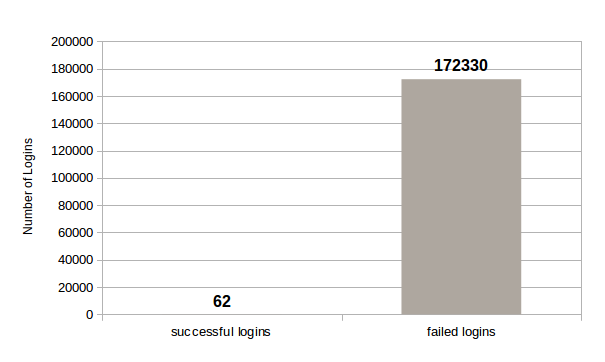
\includegraphics[scale=0.45]{login-attempts.png}
\end{figure}

Interesting fact, from the more than 172,000 failed logins are that after launching the honeypot servers to the Internet, the number of source IP addresses attacking the server were around 428. From the top 10 source IP addresses that attacked our servers we can also highlight that, in the period where blocking was still not activated, the \emph{number 1} source IP address made a brute force attack of almost \emph{32,974 login attempts}, as seen on Figure \ref{loginattempts2}. Notice that even \emph{number 10} of our Top 10 Attackers List still had the chance to launch a brute force attack of almost \emph{5,621}. A total of \emph{119,100} failed login attempts were inserted into the log files with only 10 IP addresses. 
\begin{figure}[h!]
\caption{\textbf{Top 10 IP Addresses with Number of Failed Logins}}
\label{loginattempts2}
\centering
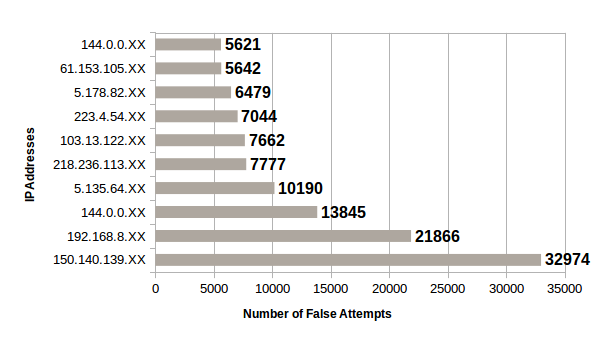
\includegraphics[scale=0.40]{false-attempts-per-ip.png}
\end{figure}
\section{Conclusions}
\label{conclusion}
After correlating all the information in the CIDS the results obtained for a brute force attack on an environment running ssh confirmed that:
\begin{itemize}
\item The anomaly-based intrusion detection rate can be increased by doing correlation of all the logs of the different network components. Correlating logs from different network entities let the framework in advanced determine possible collaborative attacks based on the failed attempts an specific source IP address is committing.
\item Based on the correlation and early discover of an attack, the framework is able to rapidly determine and confirm an attack, and also to notify the rest of network entities on the network to block the IP source address of the attacker. This process of determining an attack, filtering, identifying and notifying other entities is one the main contributions of this paper. 
\item With the process mentioned above, the IB framework is capable of reconfiguring itself and learn from the environment it is acting. This other main contribution makes the process of detection and prevention of intrusions and attacks to be intelligent. Important that no human intervention is needed to determine the right behavior of traffic for this case study.
\item The false positive rate can be decreased by knowing the exact profile of a thread of communication between the network entities. In this case study, we are following the thread of communication to establish a remote session between network entities as described in the RFC 4254 \cite{RFC4254}. 
\item In this case study, the log message was modified to be able to run scripts on it and parse the information useful to count the exact successful and failed login attempts each source IP address committed. This modification let us understand that mainly all the information we need to implement the framework was already in the environment, but did not have the correct analysis nor correlation, to be able to make it useful information to protect hosts, servers and the whole network.
\end{itemize}

As a future work, we will include more variables to determine the possibility of being part of collaborative or anomaly-distributed intrusion attacks. We will also work in making the framework to be able to reconfigure its normal profile using machine learning techniques and be able to define new collaborative or anomaly-distributed intrusion attacks. It is important to highlight that the new classification of traffic will be shared with the rest of the IDS to make a more precise binary classification in further analyses.

%\section{Acknowledgement}
%Most of the work generated here couldn't be completed without the help of DELL. Specially, the whole engagement of the company on promoting and helping academia. Special thanks and greetings to Edgar Alvarado, who was been an enthusiast for technology.
%\bigskip

\bibliographystyle{plain}
\bibliography{bib_paper_netmm2015}
\end{document}
